
Many articles introducing novel trajectory inference (TI) tools lack quantitative assessment of the accuracy of the method. Instead, they rely on anecdotal evidence to demonstrate their added value. A brief review of 75 articles reveals that only about 37\% contain a self-assessment (Figure \ref{fig:benchmarks_over_time}A,B). Peer-reviewed articles fared even worse, self-assessing in only 34\% of cases (n=55), whereas articles first published as a pre-print self-assess in 43\% of cases (n=39).

The number of datasets used and methods compared against is also below expectations (Figure \ref{fig:benchmarks_over_time}C,D). Only three TI articles feature a comparison of at least 5 methods using 5 datasets or more \cite{sharma_forksfindingorderings_2017,guo_hoplandsinglecellpseudotime_2017,parra_reconstructingcomplexlineage_2018}. In comparison, our recent benchmark of TI methods evaluated the performance 45 TI methods on 110 real and 229 synthetic datasets\cite{saelens_comparisonsinglecelltrajectory_2019}.

While self-assessments are universally biased in favour of the authors\cite{norel_selfassessmenttrapcan_2011} (intentially or not), it is dangerous and unusual to publish a computational tool without quantitatively demonstrating its performance compared to state-of-the-art methods. Indeed, our comparison demonstrated that most methods perform worse than a few baseline methods constructed by combining simple off-the-shelf algorithms such as PCA, $k$-means and MST.

In this perspective, we hypothesise that low self-assessment rates are primarily caused by a lack of a standardised problem definition, readily available benchmarking datasets, and suitable metrics. 
We elaborate on these causal reasons, and provide viable solutions for performing TI benchmarks more easily.

\begin{figure}[htb!]
	\centering
	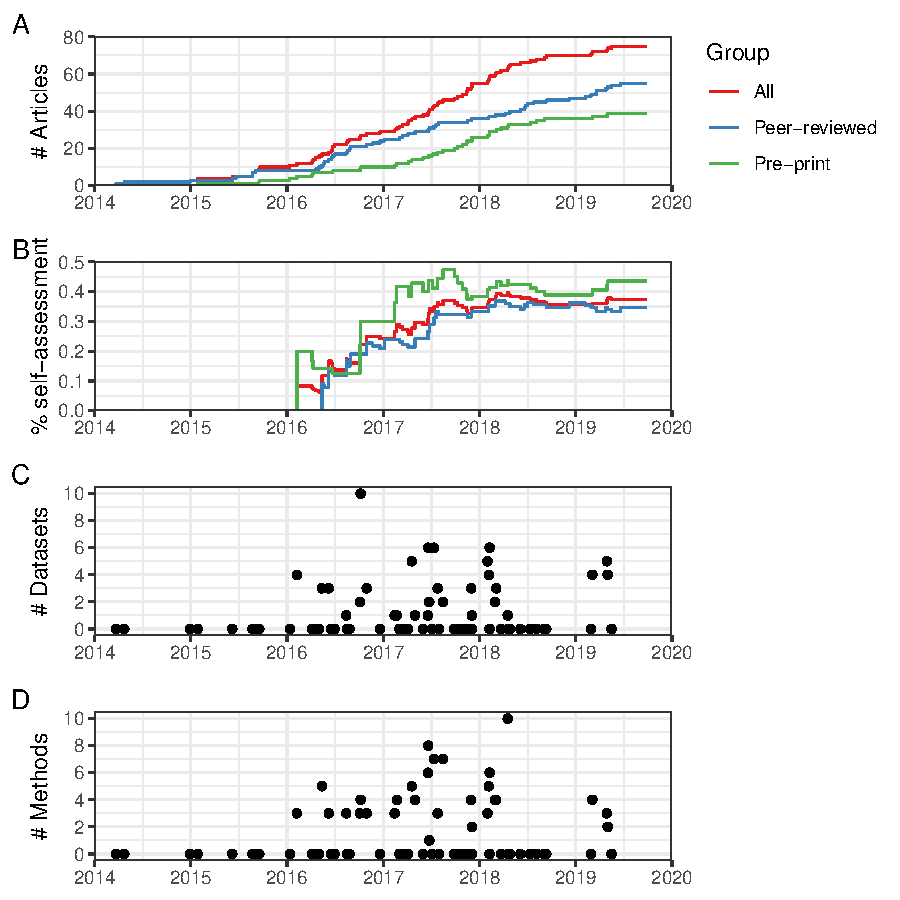
\includegraphics[width=.75\linewidth]{fig/self_assessment.pdf} 
	\caption{
		\textbf{Less than half of all TI articles perform quantitative self-assessment.} 
		\textbf{A:} Since 2016, the number of TI articles has been increasing rapidly. Note that TI methods with both a pre-print and a peer-reviewed article only count once in the overall tally.
		\textbf{B:} Less than 50\% of articles feature a self-assessment. Peer-reviewed articles self-assess only in 34\% of cases.
		\textbf{C:} The number of datasets used in each benchmark is low.
		\textbf{D:} The number of methods (inclusing itself) evaluated is low.
	}
	\label{fig:benchmarks_over_time}
\end{figure}

\section{Problem definition}
One main reason why benchmarking TI methods is difficult is due to there being slight variations 
of the problem a method is attempting to solve (Figure \ref{fig:method_types}A). For example, a method might infer linear or cyclic trajectories, or predict the probability of a cell ending up in one of several end states.

As a result, it becomes harder to discover similar methods to compare against, as certain articles might only show up with search terms such as "pseudotemporal ordering", "lineage trees" or "fate bias". For the discoverability of a new TI method, it is therefore essential to use the term "trajectory inference", or at least list it as one of the keywords. 

\begin{figure}[htb!]
	\centering
	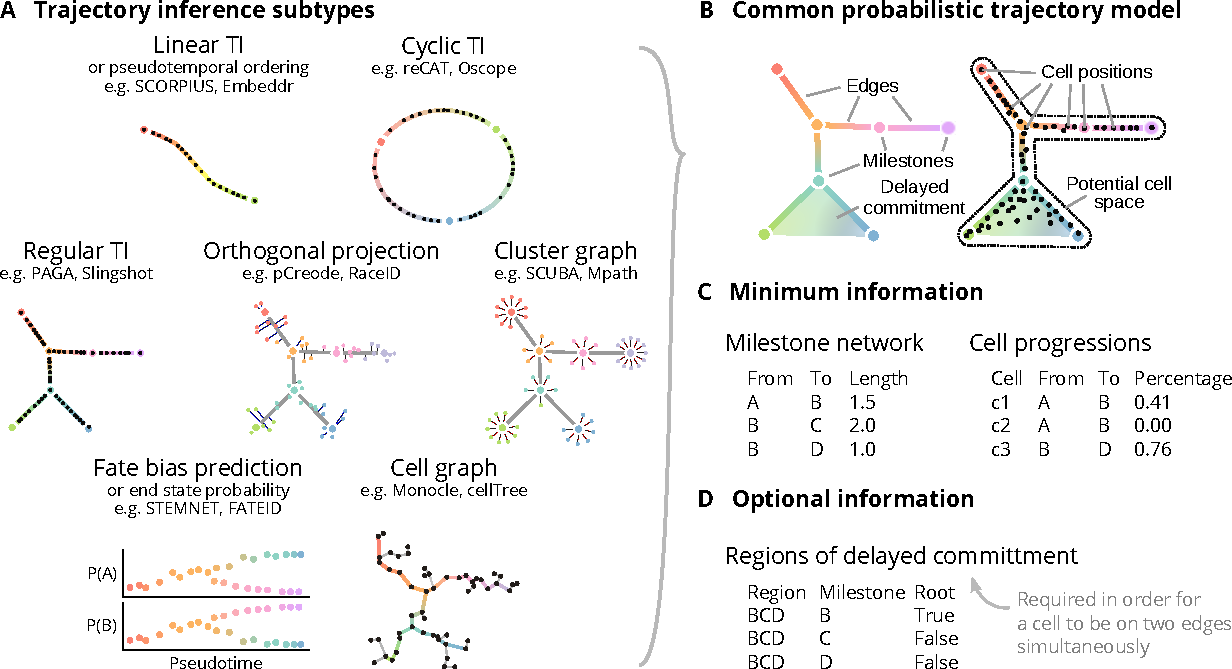
\includegraphics[width=\linewidth]{fig/method_types.pdf} 
	\caption{
		\textbf{Different forms of trajectory inference.}
		\textbf{A:} All TI methods can be categorised in one of seven subtypes in terms of its produced output \cite{saelens_comparisonsinglecelltrajectory_2019}.
		\textbf{B:} Each of these can be translated into a common format, allowing easier comparison of multiple trajectories.
		\textbf{C:} The minimum information required to describe a trajectory in this way is the milestone network -- representing transitions between cellular states -- and the cell progressions -- representing the positions of cells along the transitions.
		\textbf{D:} Optionally, regions of delayed commitment can be defined. A region of delayed commitment contain multiple transitions starting from the same milestone. This allows a TI method to assign probabilities on how likely a cell is part of one of these transitions.
	}
	\label{fig:method_types}
\end{figure}

A more significant and harder to solve problem is that the data formats produced by different methods varies greatly. This makes visualising and comparing multiple trajectories difficult, as different output types cannot be compared directly. The most commonly used and general is one where cells are positioned along a set of edges connecting milestones ("Regular TI", Figure~\ref{fig:method_types}A). 
By adding an extension to regular TI to allow for cells to be part of three or more cellular states, thereby a cell to delay its commitment toward a particular end state (Figure~\ref{fig:method_types}B). 

By adding this extension, all TI subtypes can easily be converted into the common format. Implementations of these conversions can be found in \texttt{dynwrap}\cite{dyno}. Using this standardised format allows developing reusable software for visualising and comparing trajectories from different TI methods.

\mycomment{Todo: mention containerised methods in dynmethods or simply using them as standalone containers.}

In practice, this format consists of two data structures: the milestone network specify transition between cell states, and the cell progressions specify how far along each cell has progressed along a transition (Figure~\ref{fig:method_types}C). In addition, regions of delayed commitment need to be specified, if any (Figure~\ref{fig:method_types}D). 

\mycomment{examples? elaborate? citation?}

\section{Benchmarking datasets}
Another hurdle in benchmarking trajectory inference methods is collecting datasets to benchmark against. Before 2018, there were only a handful of datasets containing complex trajectories (Figure~\ref{fig:datasets}). 

When real data is scarce, synthetic data is often used to evaluate computational methods, either standalone (n=5) or to complement real data (n=7). Most synthetic data is generated by the authors themselves (n=8), whereas some reuse datasets generated by others (n=3) or use one of the readily available simulators (n=2). To avoid introducing self-assessment bias in a benchmark, it is recommended to use readily available simulators if they fit the requirements. Examples are dyntoy \cite{saelens_comparisonsinglecelltrajectory_2019}, dyngen \cite{dyngen}, splatter \cite{zappia_splattersimulationsinglecell_2017}, and PROSSTT \cite{papadopoulos_prossttprobabilisticsimulation_2018}.

\begin{figure}[htb!]
	\centering
	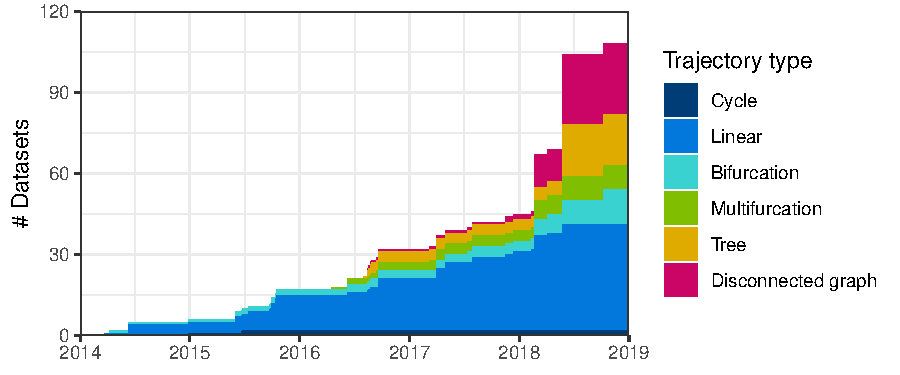
\includegraphics[width=.75\linewidth]{fig/datasets.pdf} 
	\caption{\textbf{An overview collection of real TI benchmarking datasets in function of their publication date and the topology of the trajectory.} These datasets are readily available on Zenodo\cite{cannoodt_singlecellomicsdatasets_2018}.}
	\label{fig:datasets}
\end{figure}

Benefits of synthetic data are that they offer more control over the data characteristics, and that they can be generated in large quantities. This allows to evaluate performance of a method in function of a changing parameter (e.g. dataset size or noise levels), which provides information on how well the method will work on real datasets.

A common counterargument of synthetic data is that they generate unrealistic datasets and thus provide no additional value in evaluation a method. In contrast, we argue that a good set of synthetic datasets should allow benchmarkers to verify that a method should \textit{at least} work well on the synthetic datasets, but good performance on synthetic datasets does not guarantee good performance on real datasets.

Several authors use mainly real datasets to evaluate their method, though only few use more than four datasets (n=7). 
By now, already hundreds of suitable real datasets are available from GEO and ArrayExpress (Figure~\ref{fig:datasets}). Downloading and pre-processing them requires a significant time investment, but by processing the datasets once and storing them in a single repository they can be reused for multiple purposes. Mixture control experiments\cite{tian_benchmarkingsinglecell_2019} are particularly useful in this context.

Readers are welcome to reuse (and extend) the 110 real and 229 synthetic datasets used in our comparison of TI methods\cite{saelens_comparisonsinglecelltrajectory_2019}. The datasets are hosted on Zenodo\cite{cannoodt_singlecellomicsdatasets_2018} and the scripts to process them on GitHub\footnote{\href{https://github.com/dynverse/dynbenchmark/tree/master/scripts/01-datasets}{github.com/dynverse/dynbenchmark/tree/master/scripts/01-datasets}}. Note that the ground truths of the datasets are represented using the common data structures format in the previous section.

\section{Metrics}
To evaluate a TI method, a quantitative metric is needed to compare the predicted trajectory to the ground truth trajectory. No off-the-shelf metrics exist for comparing complex multilayered data structures such as trajectories to each other.
To get around this problem, most benchmarks repurpose metrics from other domains (Figure~\ref{fig:metrics}A).

For example, most benchmarks (n=26) compare the linear pseudotime ordering of a trajectory with ground-truth information such as time time of sampling, quite often by calculating the pearson correlation. This is a good approach for comparing linear trajectories, but is not suitable as a metric for comparing non-linear trajectories (e.g. by calculating the distance from one end point of the trajectory), as this metric does not capture any differences in topology between the two trajectories (Figure~\ref{fig:metrics}B).
Several other benchmarks (n=5) use a metric typically used to compare a clustering method, by comparing a cell's assignment to the transitions of the trajectory to ground-truth information such as the cell's cell type. While this will provide some information on whether cells are grouped correctly in comparison to the ground-truth, it also does not capture topological differences between trajectories (Figure~\ref{fig:metrics}C). 

\begin{figure}[htb!]
	\centering
	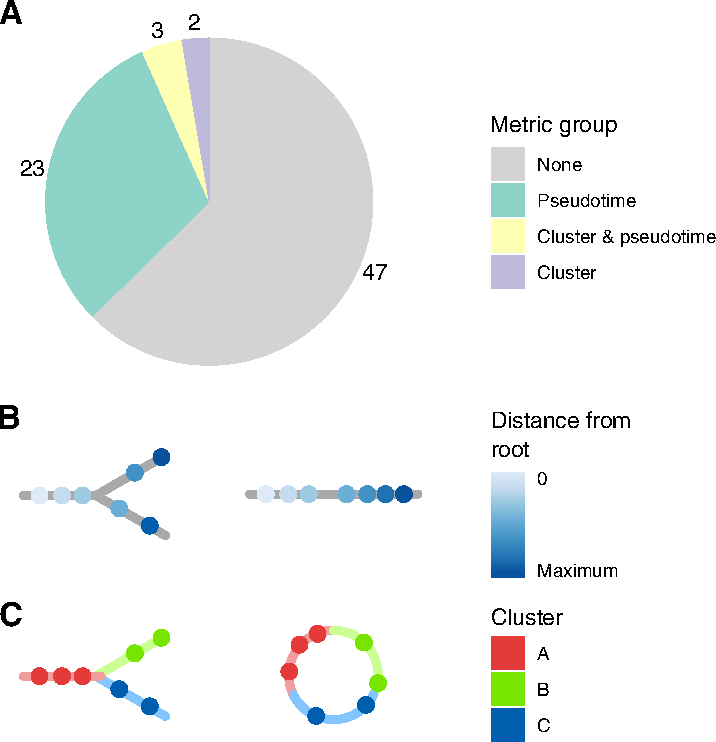
\includegraphics[width=.6\linewidth]{fig/perturbations.pdf} 
	\caption{
		\textbf{A:} Without any off-the-shelf metrics to use for evaluating TI methods, authors use metrics from other domains.
		\textbf{B:} Comparing these two trajectories using a pseudotime metric (e.g. pearson correlation) would return a perfect score, even though these two trajectories are clearly different.
		\textbf{C:} Comparing these two trajectories using a clustering metric (e.g. ARI) would also return a perfect score, even though these two trajectories are clearly different.
	}
	\label{fig:metrics}
\end{figure}

Extra credit should be given to four cases in which the robustness of methods was evaluated by comparing multiple executions of the same method\cite{haghverdi_diffusionpseudotimerobustly_2016,cannoodt_scorpiusimprovestrajectory_2016,_doesyourcode_2018,sharma_forksfindingorderings_2017,jin_scepathenergylandscapebased_2018}. Computing the robustness does not replace the necessity of a relevant metric that captures whether a predicted trajectory resembles the ground truth -- that is, a TI method can robustly make incorrect predictions and obtain high robustness scores.
In another benchmark, an internal metric is used to quantify the smoothness of gene expression along the pseudotime \cite{darocha_reconstructioncomplexsinglecell_2018} -- the idea being that good TI methods would order cells such that gene expression is smooth along the pseudotime.


In our comparison of TI methods\cite{saelens_comparisonsinglecelltrajectory_2019}, we use a metric called the \emph{geodesic correlation}. Here, two trajectories are compared by calculating the geodesic distances between pairs of cells and comparing those distance values using a Pearson correlation. Note not all pairwise distances are evaluated in this way, or the metric would not scale well to larger datasets. We also use the Hamming-Ipsen-Mikhailov (HIM) distance\cite{jurman_himglocalmetric_2015} to compare the topology of two trajectories. 

In Supplementary Note 1 of our comparison of TI methods, we describe and illustrate 10 different metrics, including the geodesic correlation metric, the HIM distance, and several clustering and internal metrics. We constructed 26 test cases (similar to Figure~\ref{fig:metrics}B,C) to assess whether a metric is able of capturing the desired information. We found that the geodesic distance passes nearly all of the test cases, using the geometric mean of different metrics performs much better.

All of these metrics are described in detail in Supplementary Note 1 and implementations are available in \texttt{dyneval}\cite{dyno}. 

\section{Guidelines for performing self-assessments}
Articles introducing novel trajectory inference methods have unfortunately been plagued by low self-assessment rates. Most articles passing peer-review do not provide quantitative evidence that their method performs well. In the previous sections, we show that this is most likely caused by differing problem statements making methods hard to compare and a lack of benchmarking datasets and relevant metrics. We provide the reader with viable solutions to each of the problems, in order to be able to benchmark their method with ease.

We wish to leave the reader with a set of guidelines on how to perform a self-assessment on the performance of their own computational method.
%refer to: \cite{norel_selfassessmenttrapcan_2011} 
%In order to alleviate the overestimation of accuracy from the many bias sources described above, we proposed a few guidelines:
%* use third‐party validation to test a model with previously unseen data
%* use more than one metric to evaluate the methods
%* report well‐performing methods even if they are not the best performers on a particular data set
%* increase the awareness of editors and reviewers that superior performance in self‐assessment is a biased demonstration of the method's value; instead, impartial assessment should be the preferred evaluation
%* Establish a scientific culture that values timely, well‐conducted follow‐up studies that confirm or refute previous results

\mycomment{Get a few guidelines from \cite{norel_selfassessmenttrapcan_2011} and \cite{weber_essentialguidelinescomputational_2019}.}


\begin{table}[h]
	\caption{\textbf{Trajectory inference method metadata.} } \label{tab:methods}
	\centering
	\tiny
	\rowcolors{2}{gray!10}{white}
\begin{tabularx}{\linewidth}{|lp{1cm}p{1cm}lXXX|}
	\hline
	id & preprint date & publication date & doi & methods & metrics & datasets \\ \hline \hline
monocle1 &  & 2014-03-23 & \doi{10.1038/nbt.2859} &  &  &  \\
wanderlust &  & 2014-04-24 & \doi{10.1016/j.cell.2014.04.005} &  &  &  \\
scuba &  & 2014-12-30 & \doi{10.1073/pnas.1408993111} &  &  &  \\
sincell & 2015-01-27 & 2015-06-22 & \doi{10.1093/bioinformatics/btv368} &  &  &  \\
nbor &  & 2015-06-08 & \doi{10.1038/ni.3200} &  &  &  \\
oscope &  & 2015-08-24 & \doi{10.1038/nmeth.3549} &  &  &  \\
cycler &  & 2015-08-24 & \doi{10.1038/nmeth.3545} &  &  &  \\
waterfall &  & 2015-09-03 & \doi{10.1016/j.stem.2015.07.013} &  &  &  \\
gpseudotime & 2015-09-15 &  & \doi{10.1101/026872} &  &  &  \\
embeddr & 2015-09-18 &  & \doi{10.1101/027219} &  &  &  \\
eclair & 2016-01-12 & 2016-05-20 & \doi{10.1093/nar/gkw452} &  &  &  \\
dpt & 2016-02-08 & 2016-08-29 & \doi{10.1038/nmeth.3971} & dpt, wishbone, monocle1 & pseudotime\_correlation, robustness\_unknown & moignard, klein, paul, synthetic\_dpt \\
pseudogp & 2016-04-05 & 2016-11-21 & \doi{10.1371/journal.pcbi.1005212} &  &  &  \\
slicer & 2016-04-09 & 2016-05-23 & \doi{10.1186/s13059-016-0975-3} &  &  &  \\
scell &  & 2016-04-19 & \doi{10.1093/bioinformatics/btw201} &  &  &  \\
wishbone &  & 2016-05-02 & \doi{10.1016/j.cell.2014.04.005} &  &  &  \\
tscan &  & 2016-05-13 & \doi{10.1093/nar/gkw430} & monocle1, tscan, waterfall, scuba, wanderlust & pseudotime\_pos & trapnell, amit, shin \\
scoup &  & 2016-06-08 & \doi{10.1186/s12859-016-1109-3} & scoup, monocle1, tscan & pseudotime\_pis & kouno, moignard, shalek \\
delorean &  & 2016-06-17 & \doi{10.1093/bioinformatics/btw372} &  &  &  \\
raceid\_stemid &  & 2016-06-21 & \doi{10.1016/j.stem.2016.05.010} &  &  &  \\
ouija & 2016-06-23 &  & \doi{10.1101/060442} &  &  &  \\
mpath &  & 2016-06-30 & \doi{10.1038/ncomms11988} &  &  &  \\
celltree &  & 2016-08-13 & \doi{10.1186/s12859-016-1175-6} & monocle1, tscan, celltree & pseudotime\_unknown & trapnell \\
wavecrest &  & 2016-08-17 & \doi{10.1186/s13059-016-1033-x} &  &  &  \\
stemnet &  & 2016-08-25 & \doi{10.1038/ncb3493} &  &  &  \\
scimitar & 2016-10-04 & 2017-01-04 & \doi{10.1142/9789813207813\_0053} & scimitar, monocle1, wanderlust & pseudotime\_correlation & synthetic\_scimitar, synthetic\_scimitar \\
scorpius & 2016-10-07 &  & \doi{10.1101/079509} & scorpius, wanderlust, monocle1, waterfall & pseudotime\_cos, robustness\_cva & schlitzer, buettner, shalek, shalek, shalek, trapnell, kowalczyk, kowalczyk, kowalczyk, kowalczyk \\
scent &  & 2016-10-30 & \doi{10.1038/ncomms15599} & scent, slice, stemid & pseudotime\_wilcox, pseudotime\_auc & chu, trapnell, treutlein \\
slice &  & 2016-12-19 & \doi{10.1093/nar/gkw1278} &  &  &  \\
topslam & 2017-02-13 &  & \doi{10.1101/057778} & monocle1, wishbone, topslam & pseudotime\_correlation & synthetic\_topslam \\
monocle2 & 2017-02-21 & 2017-07-20 & \doi{10.1038/nmeth.4402} & monocle1, monocle2, dpt, wishbone & pseudotime\_correlation, branch\_ari & paul \\
gpfates &  & 2017-03-03 & \doi{10.1126/sciimmunol.aal2192} &  &  &  \\
mfa &  & 2017-03-15 & \doi{10.12688/wellcomeopenres.11087.1} &  &  &  \\
tasic &  & 2017-04-04 & \doi{10.1093/bioinformatics/btx173} &  &  &  \\
somsc & 2017-04-05 &  & \doi{10.1101/124693} &  &  &  \\
slingshot & 2017-04-19 & 2018-06-19 & \doi{10.1186/s12864-018-4772-0} & slingshot, monocle1, monocle2, dpt, tscan & pseudotime\_correlation & synthetic\_splatter, synthetic\_splatter, synthetic\_splatter, synthetic\_splatter, synthetic\_splatter \\
sctda &  & 2017-05-01 & \doi{10.1038/nbt.3854} & sctda, wishbone, slicer, dpt & pseudotime\_correlation & synthetic\_sctda \\
uncurl & 2017-05-31 &  & \doi{10.1101/142398} &  &  &  \\
recat &  & 2017-06-19 & \doi{10.1038/s41467-017-00039-z} & recat, scuba, monocle1, tscan, wishbone, dpt & pseudotime\_correlation, pseudotime\_custom & buettner \\
forks & 2017-06-20 &  & \doi{10.1101/132811} & forks, monocle2, scuba, tscan, waterfall, dpt, gpfates, slicer & pseudotime\_correlation, robustness\_stdev & windram, deng, guo, klein, amit, petropoulos \\
matcher &  & 2017-06-24 & \doi{10.1186/s13059-017-1269-0} & matcher & pseudotime\_correlation & angelmueller, synthetic\_matcher \\
phenopath & 2017-07-06 & 2018-06-23 & \doi{10.1101/159913} &  &  &  \\
hopland &  & 2017-07-12 & \doi{10.1093/bioinformatics/btx232} & hopland, wanderlust, monocle1, topslam, scuba, wishbone, dpt & pseudotime\_correlation & guo, deng, yan, amit, islam, synthetic\_topslam \\
soptsc & 2017-07-26 & 2019-06-20 & \doi{10.1093/nar/gkz204} & soptsc, monocle2, dpt & pseudotime\_correlation & guo, klein, shalek \\
pba &  & 2017-07-30 & \doi{10.1073/pnas.1714723115} &  &  &  \\
brgps & 2017-08-15 &  & \doi{10.1101/167684} & brgps, grandprix, monocle2, scuba, slicer, tscan, wishbone & pseudotime\_correlation & guo, guo \\
wot & 2017-09-27 & 2019-02-07 & \doi{10.1016/j.cell.2019.01.006} &  &  &  \\
treetop & 2017-10-10 &  & \doi{10.1101/200923} &  &  &  \\
paga & 2017-10-27 & 2019-03-19 & \doi{10.1186/s13059-019-1663-x} &  &  &  \\
fateid & 2017-11-11 & 2018-04-09 & \doi{10.1038/nmeth.4662} &  &  &  \\
pseudodynamics & 2017-11-14 &  & \doi{10.1101/219188} &  &  &  \\
pcreode &  & 2017-11-15 & \doi{10.1016/j.cels.2017.10.012} &  &  &  \\
icpsc &  & 2017-11-30 & \doi{10.1038/s41467-017-01860-2} & icpsc, wishbone, monocle2, dpt & pseudotime\_correlation & sun, trapnell, yao \\
grandprix & 2017-12-03 & 2018-07-02 & \doi{10.1101/227843} & delorean, grandprix & pseudotime\_correlation & windram \\
cshmm & 2017-12-03 & 2019-04-30 & \doi{10.1093/bioinformatics/btz296} &  &  &  \\
calista & 2018-01-31 &  & \doi{10.1101/257550} & monocle2, calista, dpt & pseudotime\_correlation & moignard, bargaje, treutlein, chu, synthetic\_calista \\
scepath &  & 2018-02-05 & \doi{10.1093/bioinformatics/bty058} & scepath, monocle1, monocle2, tscan, dpt & pseudotime\_correlation, robustness\_correlation & yan, treutlein, treutlein, trapnell \\
merlot & 2018-02-08 &  & \doi{10.1101/261768} & merlot, dpt, slicer, monocle2, slingshot, tscan & branch\_mi, pseudotime\_correlation & paul, guo, velten, synthetic\_prosstt, synthetic\_prosstt, synthetic\_splatter \\
gpseudorank & 2018-02-08 & 2018-07-25 & \doi{10.1093/bioinformatics/bty664} &  &  &  \\
cellrouter &  & 2018-03-01 & \doi{10.1038/s41467-018-03214-y} & monocle2, dpt, wishbone, waterfall & internal\_autocorrelation & paul, olsson \\
densitypath & 2018-03-05 & 2018-12-07 & \doi{10.1093/bioinformatics/bty1009} & monocle2, wishbone, dpt, densitypath & branch\_ari, pseudotime\_correlation & petropoulos, synthetic\_phate, synthetic\_topslam \\
topographer & 2018-03-23 &  & \doi{10.1101/251207} &  &  &  \\
stream & 2018-04-18 & 2019-04-23 & \doi{10.1038/s41467-019-09670-4} & stream, sctda, wishbone, slicer, monocle2, dpt, tscan, scuba, mpath, gpfates & pseudotime\_correlation & synthetic\_sctda \\
elpigraph & 2018-04-20 &  & arXiv:\href{https://arxiv.org/abs/1804.0758}{1804.0758} &  &  &  \\
urd &  & 2018-04-26 & \doi{10.1126/science.aar3131} &  &  &  \\
celltrails &  & 2018-06-05 & \doi{10.1016/j.celrep.2018.05.002} &  &  &  \\
ddd & 2018-07-12 &  & \doi{10.1101/367789} &  &  &  \\
palantir & 2018-08-05 & 2019-03-21 & \doi{10.1038/s41587-019-0068-4} &  &  &  \\
confess & 2018-09-04 &  & \doi{10.1101/407932} &  &  &  \\
graphddp &  & 2018-09-11 & \doi{10.1038/s41467-018-05988-7} &  &  &  \\
monocle3 &  & 2019-02-28 & \doi{10.1038/s41586-019-0969-x} &  &  &  \\
gpseudoclust & 2019-03-05 &  & \doi{10.1101/567115} & gpseudoclust, monocle2, delorian, slicer & cluster\_ari, cluster\_fmi, cluster\_nmi & sasagawa, shalek, synthetic\_gpseudoclust, synthetic\_gpseudoclust \\
psupertime & 2019-04-29 &  & \doi{10.1101/622001} & monocle2, slingshot, psupertime & pseudotime\_correlation & enge, qiu, petropoulos, li, treutlein \\
cyclum & 2019-05-02 &  & \doi{10.1101/625566} & cyclum, recat & cluster\_accuracy & buettner, mcdavid, mcdavid, mcdavid \\
sinova &  & 2019-05-17 & \doi{10.1016/j.celrep.2016.04.043} &  &  &  \\
\hline
\end{tabularx}
\end{table}